The Van der Waals (vdW) force originates from nonlocal correlations in the quantum motion of electrons, and give rise to a wide spectrum of physical phenomena, ranging from attraction between two atoms~\citep{LondonZP30} to the macroscopic Casimir effect~\citep{JaffePRD05}.
They dictate thermodynamic properties of many molecular solids, layered and nanostructured materials, and biological compounds, and govern processes such as molecular adsorption and self-assembly, including most biological processes.
As a result, vdW interactions have been, and are increasingly so, one of the prime targets of material modeling, which has led to a plethora of approaches that either treat vdW forces implicitly or model them explicitly~\citep{KlimesJCP12,GrimmeCR16,HermannCR17}.
These include quantum Monte--Carlo~\citep{AmbrosettiJPCL14} (QMC), coupled clusters~\citep{YangS14}, random-phase approximation~\citep{LuPRL09}, nonlocal density functionals~\citep{DionPRL04,VydrovPRL09}, and coarse-grained approaches, which range from pairwise~\citep{GrimmeJCC04,BeckeJCP07,TkatchenkoPRL09} to many-body models~\citep{TkatchenkoPRL12,SilvestrelliJCP13}.
From theoretical perspective, this status quo is undesirable, because different models often give disparate pictures of the nature of vdW forces, which leads to incoherent understanding of vdW interactions in molecules and materials.
From practical perspective, the three main characteristics of a method are its applicability, accuracy, and computational efficiency, and so far, no single method has satisfied all three requirements with respect to vdW forces to such a degree, that it would be reliably applicable to all the relevant types of materials.
For instance, QMC and coupled clusters are limited by computational efficiency, pairwise approaches lack in accuracy for nanostructured and supramolecular compounds, and coarse-grained models have qualitative problems with description of ionic and hybrid metal-organic systems.

In this Letter, we present a unified density-functional model of vdW interactions that combines ingredients from nonlocal functionals and coarse-grained models, inheriting broad applicability of the former and good accuracy of the latter, while retaining the computational efficiency of both.
We integrate the polarizability functional of \citet{VydrovPRA10} (VV), normalization to reference free-atom vdW parameters coined by the exchange-hole dipole moment model~\citep{BeckeJCP06} and the vdW model of \citet{TkatchenkoPRL09} (TS), the idea of normalization to jellium via a zero-gradient limit from the VV10 nonlocal functional~\citep{VydrovJCP10a}, and the Hamiltonian form of the many-body dispersion (MBD) model~\citep{TkatchenkoJCP13}.
Compared to the range-separated self-consistently screened (rsSCS) variant of MBD~\citep{AmbrosettiJCP14}, the use of the VV polarizability functional in the new model enables consistent treatment of ionic compounds, normalization to free-atom reference values balances the accuracy of the VV polarizability across the periodic table, while normalization to jellium enables effective modeling of adsorption on metallic surfaces~\citep{RuizPRL12}.
Furthermore, the VV functional---unlike approaches based on Hirshfeld volumes---
is able to capture short-range many-body polarization effects, so that the short-range screening of atomic polarizabilities is not needed in the new model, reducing the overall computational cost by an order of magnitude compared to MBD@rsSCS\@.
In our consideration, a similar level of empiricism is involved in the construction of the new model compared to MBD@rsSCS\@.
On one hand we remove the need for tabulated reference vdW radii and for the short-range screening, on the other we introduce new mechanisms that contain some quantitative empirical choices.
However, these choices are motivated by well-understood goals, and can be justified qualitatively without resorting to empirical arguments.
We demonstrate on a series of benchmark calculations that our new model enables for the first time consistent treatment of vdW interactions in covalent, ionic, and hybrid metal-organic interfaces by a single method, while achieving the accuracy of the best approaches for each of these material types.

The central proposition of the new model, dubbed MBD@VV, is to parameterize the Hamiltonian of the MBD model with the VV polarizability functional.
In general, each vdW model consists of two main ingredients: a model for the noninteracting polarization response and the model for long-range coupling of this response.
The shortcomings of many existing vdW approaches in description of ionic compounds and hybrid interfaces do not originate from the model for the coupling, but rather from the model for polarization response.
Its improvement is the main focus of this work.
In the case of coarse-grained models, such as MBD, the model for the response translates into a model for static polarizabilities $\alpha_{0,i}$ and $C_{6,i}$ coefficients of the interacting fragments (usually atoms).
In MBD@VV, we parametrize the response of atoms by coarse-graining the VV polarizability density to Hirshfeld fragments~\citep{HirshfeldTCA77,SatoJCP09,SatoJCP10}.
The VV functional is a semilocal functional of the electron density $n(\mathbf r)$, which models local isotropic dynamic polarizability density,
\begin{equation}
   \alpha^\text{VV}[n](\mathbf r,\mathrm iu)=\frac{n(\mathbf r)}{\frac{4\pi}3n(\mathbf r)+C\frac{{|\boldsymbol\nabla n(\mathbf r)|}^4}{n{(\mathbf r)}^4}+u^2}
   \label{eq:vv-functional}
\end{equation}
where $\mathrm iu$ is imaginary frequency and $C$ is an empirical parameter fitted to reproduce a reference set of $C_6$ coefficients.
The atomic dynamic polarizabilities are obtained by integrating the polarizability density with Hirshfeld weights $w_i^\text{H}(\mathbf r)$,
\begin{equation}
  \alpha_i^\text{VV}(\mathrm iu)=\int\mathrm d\mathbf r\,w_i^\text{H}(\mathbf r)\alpha^\text{VV}[n](\mathbf r,\mathrm iu)
\end{equation}
The $C_6$ coefficients are calculated directly from $\alpha_i(\mathrm iu)$ via the Casimir--Polder formula,
\begin{equation}
  C_{6,i}^\text{VV}=\frac3\pi\int_0^\infty\mathrm du\,\alpha_i^\text{VV}{(\mathrm iu)}^2
\end{equation}
Unlike in approaches that use Hirshfeld fragments to define atomic volumes, the particular choice of the atomic partitioning in MBD@VV is mostly inconsequential, because it only influences local redistribution of the polarizability between atoms---not total polarizability, nor polarizability distribution over larger length scales.
Our approach is also different from that of \citet{SilvestrelliPRL08}, in which the electron density is coarse-grained first and a polarizability functional is evaluated over those fragment densities.
Such an approach does not conserve the total polarizability.

Already this initial combination of the MBD model and VV polarizability functional gives a substantial improvement in description of ionic systems over MBD@rsSCS, thanks to the versatility of the VV functional.
However, it suffers from two theoretical shortcomings.
First, the polarizability functional is in no way guaranteed to be exact for free atoms across the periodic table, which is a basic requirement for a highly accurate and general model.
Second, when combined with semilocal density-functional theory (DFT), it suffers from double-counting of electron correlation in regions of slowly-varying electron density.
To solve these two issues, we borrow two techniques from the TS model and from the VV10 nonlocal functional.
First, we normalize the atomic VV polarizabilities and $C_6$ coefficients to reproduce the respective exact quantities for free atoms.
Second, we normalize MBD@VV such that it gives zero vdW energy for jellium by subtracting the portion of the polarizability that comes from metallic electron density regions.

\begin{figure}[t!]
\centering
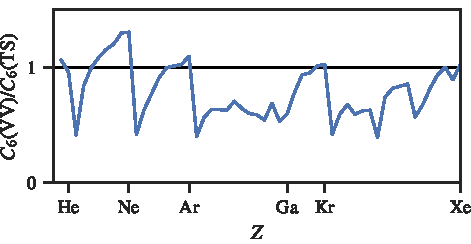
\includegraphics{../media/vv-periodic-table.pdf}
\caption{\textbf{Relative errors in VV polarizabilities of free atoms for first 54 elements.}
The reference values are the same as used in the TS method.
}\label{fig:vv-periodic-table}
\end{figure}

The VV polarizability functional is only approximate, which is manifest already for free-atom polarizabilities and $C_6$ coefficients, where accurate reference values are known (Figure~\ref{fig:vv-periodic-table}).
Whereas the VV functional reproduces atoms of nonmetallic elements quite accurately (especially the important carbon atom with error in the $C_6$ coefficient less than 2\%), the polarizabilities and $C_6$ coefficients of atoms of metallic elements are substantially underestimated.
To mitigate this error, we normalize the VV atomic quantities with the ratio of the free-atom polarizabilities and $C_6$ coefficients as calculated by the VV functional and as obtained from accurate reference calculations,
\begin{equation}
  \alpha_{0,i}^\text{rVV$'$}=\alpha_{0,i}^\mathrm{VV'}\frac{\alpha_{0,i}^\text{ref,free}}{\alpha_{0,i}^\text{VV$'$,free}},\quad
  C_{6,i}^\text{rVV$'$}=C_{6,i}^\mathrm{VV'}\frac{C_{6,i}^\text{ref,free}}{C_{6,i}^\text{VV$'$,free}}
\end{equation}
This correction assumes that any error in the VV functional is at least partially transferable from free atoms to atoms in compounds.
Alternatively, the normalization can be seen as a modification of the TS approach~\citep{TkatchenkoPRL09}, in which the ratios of Hirshfeld volumes are replaced with ratios of VV polarizabilities and $C_6$ coefficients.

% TODO
% As part of the normalization, we reoptimize the $C$ parameter in the VV functional on the same set of $C_6$ coefficients used in the TS method.
% The original formulation of the VV polarizability functional used $C=0.0089$~\citep{VydrovPRL09}, but was later reparametrized by the authors themselves to $C=0.0093$~\citep{VydrovJCP10a}.
% In both cases, the reference sets of $C_6$ coefficients used for the parametrization contained also atoms of metallic elements, which are severely underestimated by the VV functional (Figure~\ref{fig:vv-periodic-table}), and this pushed the parameter $C$ to lower values.
% The TS reference set contains mostly organic compounds, and this results in the higher value of $C=0.0101$.
% This makes the metallic elements even more underestimated by the VV functional, but that is not an issue in our approach because of to the normalization to free atoms.

Many exchange--correlation (XC) functionals are exact for jellium by construction, even though the portion of electron correlation coming from plasmons is long-ranged and should not in principle be accounted for by semilocal XC functionals.
As a result of this construction, most XC functionals describe accurately the electron correlation \emph{within} slowly-varying density regions, such as those found in metals, and no addition of vdW forces is needed in those cases.
This is unlike in all other cases, where semilocal functionals neglect long-range vdW interactions.
Furthermore, the interactions \emph{between} such regions and other regions of the electron density are effectively screened by the conducting electrons.
At the same time, these metallic-density regions contribute dominantly to the polarizability in the VV functional (in principle the local polarizability of a conductor should be infinite) and hence to the vdW energy in any vdW model, in which the VV functional would be used directly.
When combined with semilocal DFT, this would result in overpolarization and overbinding of bulk metals as well as of adsorbates on metallic surfaces.
To avoid this double-counting of the long-range electron correlation, the VV10 nonlocal functional subtracts the limit of itself as the density gradient approaches zero in the final VV10 vdW energy expression, such that the vdW energy is equal to zero for jellium,
\begin{equation}
  E_\text{vdW}^\text{VV10} = E^\text{VV10}[n]-\big(E^\text{VV10}|_{\boldsymbol\nabla n\rightarrow0}\big)[n]
\end{equation}
Such an approach cannot be used directly in a many-body model such as MBD, because unlike in a pairwise model the many-body vdW energy is not linear in the polarizability.
This would result in all the nonlinear contributions, which can be dominating in a highly polarizable system such as a metal, not being subtracted by the zero-gradient limit.
Instead, we devised an alternative construction.

Rather than evaluating the interaction of the metallic-density regions and than subtracting it, as in VV10, we do not evaluate it in the first place by smoothly cutting of the contribution of these regions to the polarizability.
These regions can be distinguished using the combination of two local dimensionless electron-density descriptors: the reduced gradient $s$ and the iso-orbital indicator $\chi$~\citep{BeckeJCP90,KummelMP03,SunPRL13},
\begin{equation}
  s[n]=\frac{|\boldsymbol\nabla n|}{2{(3\pi^2)}^\frac13n^\frac43},\qquad
  \chi[n]=\frac{\tau^\text{KS}[n]-\tau^\text{W}[n]}{\tau^\text{unif}[n]}
\end{equation}
where $\tau[n]=\sum_i|\boldsymbol\nabla\phi_i|^2/2$ is the positive kinetic energy density of occupied orbitals $\phi_i$, which for single-orbital densities reduces to the von Weizsäcker kinetic energy density, $\tau^\text W[n]=|\boldsymbol\nabla n|^2/8n$, and for jellium to $\tau^\mathrm{unif}[n]=3(3\pi^2)^{2/3}n^{5/3}/10$.  % chktex 3
The density gradient alone is not sufficient to characterize metallic density.
In particular, both $s\sim0$ and $\chi\sim1$ must be true for density to be metallic, whereas $s\sim0$ and $\chi\sim0$ corresponds to centers of covalent bonds (dominated by a single bonding orbital) and $s\sim0$ and $\chi\gg1$ signifies overlaps of electron-density tails that occur between noncovalently bound systems.
Since the normalization of VV10 to jellium uses only the density gradient, it partially omits also contributions from covalent bonds.
By using the iso-orbital indicator, we can make MBD@VV more precise in this regard.

\begin{figure}[t!]
\begin{tikzpicture}
\node[below right] at (0,0) {\bfseries a};
\node[below right, inner sep=0pt] at (0,0) {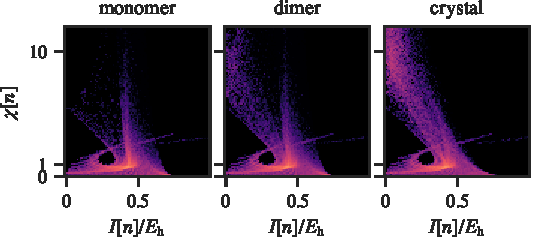
\includegraphics{../media/benzene.pdf}};
\node[below right] at (0,-4.3) {\bfseries b};
\node[below right, inner sep=0pt] at (0,-4.3) {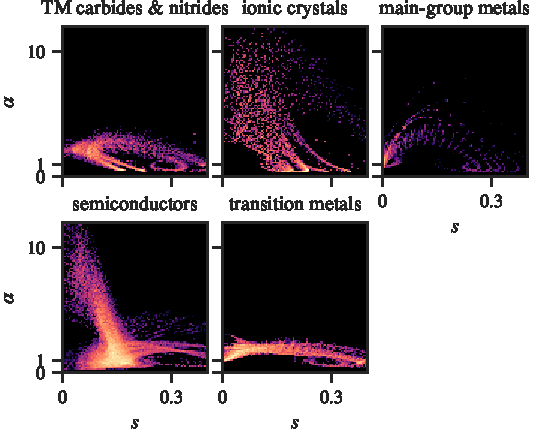
\includegraphics{../media/solids-hists.pdf}};
\end{tikzpicture}
\caption{\textbf{Polarizability distributions of reduced gradient $s$ and iso-orbital indicator $\chi$.}
Precisely, the plotted distributions are $\alpha^\text{VV}(s',\chi')=\int\mathrm d\mathbf r\delta(s(\mathbf r)-s')\delta(\chi(\mathbf r)-\chi')\alpha^\text{VV}(\mathbf r)$ such that the total polarizability is equal to $\iint\mathrm ds\mathrm d\chi\,\alpha^\text{VV}(s,\chi)$.
(\textbf a) Benzene monomer, dimer, and crystal.
Each distribution is normalized to one benzene molecule.
(\textbf b) 63 simple solids divided to five groups (see Supplementary Material for details).
Each distribution is normalized to 62 (a.\,u.), the VV polarizability of a benzene monomer, to share a single color scale with \textbf{a}.
}\label{fig:pol-hists}
\end{figure}

Figure~\ref{fig:pol-hists}a presents polarizability distributions of $s$ and $\chi$ in benzene compounds and in a set of simple solids, and shows that they are very sensitive to the nature of the bonding in a molecule or material.
In an organic molecule such as benzene (Figure~\ref{fig:pol-hists}a), the vast majority of the polarizability
comes from electron density with $s>0.1$ while the small remainder comes
from low-gradient regions with $\chi<1$.
With the introduction of intermolecular interactions in the benzene dimer and crystal, a significant additional amount of polarizability comes from regions with $\chi\gg1$, despite the electron density being low in such regions.
A richer spectrum of patterns can be found in simple solids (Figure~\ref{fig:pol-hists}b).
Most similar to the benzene compounds is the group of semiconductors.
In contrast, the vast majority of the polarizability in main-group metals comes from jellium-like regions near $(s,\chi)=(0,1)$, as expected.
In transition metals, the polarizability is distributed over a wider range of the reduced gradient along the $1<\chi<2$ strip, with a larger part still coming from low-gradient regions.
These features are largely shared by the transition-metal carbides and nitrides, but notably the near neighborhood of $(s,\chi)=(0,1)$ does not contribute in those systems.
In simple ionic solids, which do not feature covalent bonds, most of the
polarizability comes from single-orbital regions ($\chi<1$), although a
significant amount also comes from noncovalent orbital-overlap regions.

Based on these numerical results, we devised a smooth cutoff function $0\leq g(s,\chi)\leq 1$ of the two density descriptors that distinguishes the nonmetallic density regions, and define the nonmetallic portion of the polarizability density as
\begin{equation}
  \alpha^\mathrm{VV'}[n]=g(s,\chi)\alpha^\text{VV}[n]
\end{equation}
The exact shape of the cutoff function is to a certain degree arbitrary (the analytical form is presented in the Supplementary Material), but thanks to the unambiguous distinction in the polarizability distributions between organic compounds and metals, the results are not too sensitive to a particular choice.
In general terms, the cutoff function can be characterized as being zero in the largest possible region around $(s,\chi)=(0,1)$ without affecting the polarizabilities of organic compounds.
This way, the effective polarizability of a simple metal such as lithium is close to zero in our model, as is the vdW energy, whereas the difference between VV$'$ and VV polarizabilities is less than 2\% on average for organic molecules (the S66 set).

\begin{figure}[t!]
\centering
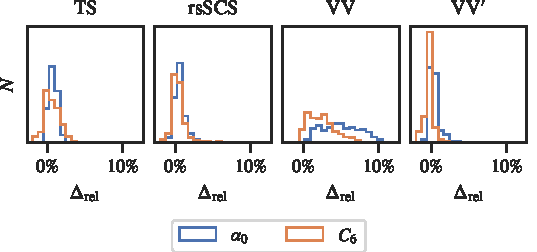
\includegraphics{../media/pol-shifts.pdf}
\caption{\textbf{Distributions of relative changes in atomic polarizabilities and $C_6$ coefficients from monomers to dimers.}
The distributions are calculated over all atoms from all complexes in the S66 data set.
}\label{fig:pol-shifts}
\end{figure}

Apart from proper treatment of metals, we use the cutoff function for another purpose.
When molecules are brought together to form vdW-bound compounds, the introduction of density-tail overlaps significantly increases the polarizability when using a model such as the VV functional (Figure~\ref{fig:pol-hists}a).
For instance, the VV polarizability per molecule goes from 62 (a.\,u.) in benzene monomer, to 67 in benzene dimer, to 92 in benzene crystal.
This effect is an artifact of the VV functional that causes increasingly large vdW-bound systems to be overbound.
To eliminate this issue, we extend the region in which the cutoff function $g$ is zero to all low-gradient regions with $\chi>1$.
This does not affect the polarizabilities of organic monomers, but ensures that the increase in polarizability from monomers to dimers is less than 1\% on average (Figure~\ref{fig:pol-shifts}).

The static polarizabilities and $C_6$ coefficients calculated as described above are then put into the MBD model to obtain the vdW energy.
The MBD Hamiltonian describes a system of charges in harmonic potentials---Drude oscillators---characterized by their static polarizabilities $\alpha_{0,i}$ and resonance frequencies $\omega_i=4C_{6,i}/3\alpha_{0,i}^2$, and interacting via a long-range dipole potential $\mathbf T^\mathrm{lr}(\mathbf R)\equiv f(R)\mathbf T(\mathbf R)$,
\begin{multline}
  H^\text{MBD}(\{\alpha_{0,i},\omega_i\})=\sum_i-\frac12\nabla_{\xi_i}^2+\sum_i\frac12\omega_i^2\xi_i^2 \\
  +\frac12\sum_{ij}\omega_i\omega_j\sqrt{\alpha_{0,i}\alpha_{0,j}}\boldsymbol{\xi}_i\cdot\mathbf T^\mathrm{lr}_{ij}\boldsymbol{\xi}_j
\end{multline}
where $\boldsymbol\xi_i\equiv\sqrt{m_i}\mathbf x_i$ are mass-weighted displacements of the charges.
To calculate the vdW energy, each oscillator is parametrized such that it models the polarization response of a single atom in a molecule or material.
The interaction energy of this model system---the vdW energy---is then readily obtained by direct diagonalization of the Hamiltonian.

In MBD@VV, we use the same form of the long-range coupling $\mathbf T^\text{lr}$ as the MBD@rsSCS variant~\citep{AmbrosettiJCP14}, but with a different definition of the vdW radii.
Rather than using tabulated free-atom vdW radii, we use the simple formula for a vdW radius of \citet{FedorovPRL18}, and rather than with ratios of Hirshfeld volumes, these free-atom vdW radii are scaled with the ratios of VV polarizability of an atom in a compound and that of a free atom,\begin{equation}
  R_i^\text{vdW}=\tfrac52{(\alpha_{0,i}^\text{ref,free})}^\frac17{\left(\frac{\alpha_i^\mathrm{VV'}}{\alpha_i^\text{VV$'$,free}}\right)}^\frac13
\end{equation}

\begin{figure}[t!]
\centering
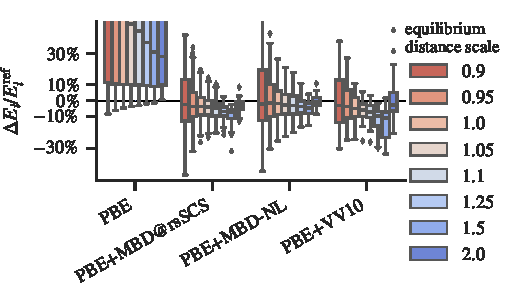
\includegraphics{../media/s66-errors.pdf}
\caption{\textbf{Distributions of relative errors in binding energies on the S66$\times$8 set.}
}\label{fig:s66-errors}
\end{figure}

\begin{figure}[t!]
\centering
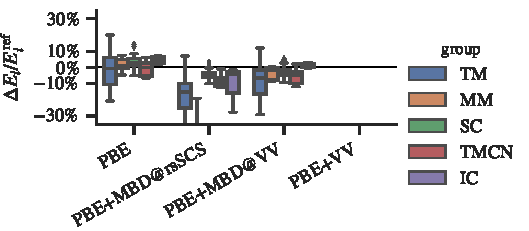
\includegraphics{../media/solids-errors.pdf}
\caption{\textbf{Distributions of relative errors in binding energies on the set of 63 solids.}
}\label{fig:solids-errors}
\end{figure}

\begin{figure}[t!]
\centering
\includegraphics{../media/silver-benzene.pdf}
\caption{\textbf{Binding energy of a single benzene molecule on a silver surface.}
}\label{fig:silver-benzene}
\end{figure}

\begin{table*}[t!]
\centering
\caption{\textbf{Performance on vdW benchmark data sets.}}\label{tab:performance}
\begin{tabular}{l*{6}{S[
  table-format=2.1,
  table-align-text-post=false,
  table-space-text-post=\%,
]}}
\toprule
XC & \multicolumn3c{MARE$^\text{a}$} & \multicolumn3c{MRE$^\text{b}$} \\
& {S66} & {X23} & {S12L} & {S66} & {X23} & {S12L} \\
\midrule
PBE & 57\% & 60\% & 82\% & 57\% & 60\% & 82\% \\
PBE+MBD@rsSCS & 8.4\% & 6.4\% & 5.3\% & -3.1\% & -3.4\% & -1.4\% \\
PBE+MBD@VV & 8.8\% & 7.0\% & 10\% & -0.4\% & 4.9\% & 8.5\% \\
PBE+VV & 9.9\% & 15\% & 15\% & -6.1\% & -15\%  & -15\% \\
\midrule
PBE0 &&&&&& \\
PBE0+MBD@rsSCS & 7.6\% & 5.4\% & 6.5\% & -1.1\% & -1.7\% & -4.4\% \\
PBE0+MBD@VV &&&&&& \\
PBE0+VV & 8.3\% & 15\% & 20\% & -5.3\% & -15\%  & -20\% \\
\bottomrule
\end{tabular}

\small
$^\text{a}$Mean absolute relative error.
$^\text{b}$Mean relative error.
\end{table*}

Next, we briefly describe several benchmark tests of the MBD@VV model, with details about the calculations, more detailed results, and additional tests reported in the Supplemental Material.
The performance on a set of small organic dimers (S66) is nearly identical to that of MBD@rsSCS (Figure~\ref{fig:s66-errors}), which is already excellent for a DFT+vdW approach.
In contrast, the errors in lattice energies of 63 simple solids are reduced drastically when MBD@rsSCS is replaced by MBD@VV (Figure~\ref{fig:solids-errors}).
This improvement comes mainly from the errors on metals and ionic solids, which PBE+MBD@rsSCS overbinds by tens of percent, whereas plain PBE performs reasonably well, and MBD@VV even slightly improves it.
PBE+MBD@VV still somewhat overbinds the metals compared to PBE, but this can be expected, because MBD@VV adds the nonlocal correlation between the bound nonconducting electrons of the metallic ions, which is missing in the PBE description, yet PBE does not underbind the metals.
The same holds for transition-metal carbides and nitrides.
Ionic solids are underbound by 4\% with PBE, which is reduced nearly to zero when the missing nonlocal correlation is added by MBD@VV, whereas MBD@rsSCS overbinds some of the ionic solids substantially.
The performance of MBD@VV on semiconductors is similar to that of MBD@rsSCS\@.

The overall performance on the S66 set, a set of organic molecular crystals (X23), and a set of supramolecular complexes (S12L) is summarized in Table~\ref{tab:performance}.
On X23, the performance of MBD@VV is similar to that of MBD@rsSCS, but rather than somewhat overbinding the crystals as PBE+MBD@rsSCS does, PBE+MBD@VV underbinds them by a similar magnitude.
On S12L, the accuracy of PBE+MBD@VV is reduced compared to PBE+MBD@rsSCS, going from 5\% to 10\%.
This results from underbinding of the $\mathrm\pi$--$\mathrm\pi$ complexes.

Benzene on silver\ldots
